\subsection{FAST - Features from Accelerated Segment Test}


FAST � um m�todo de reconhecimento baseado em detec��o de
arestas originalmente desenvolvido por Edward Rosten e Tom Drummond 
\cite{FAST}. A maior promessa do m�todo � a efici�ncia computacional. O m�todo considera um c�rculo
de dezesseis pixels ao redor da aresta considerada p.
O detector original \cite{FusingPoints},\cite{VideoAnotation} classifica
\emph{p} como uma aresta se existirem \emph{n} pixels cont�guos em um c�rculo
que s�o mais brilhantes do que o pixel candidato de intensidade Ip mais um threshold t ou mais escuros do que Ip-t

 \begin{figure}[H]
\centering
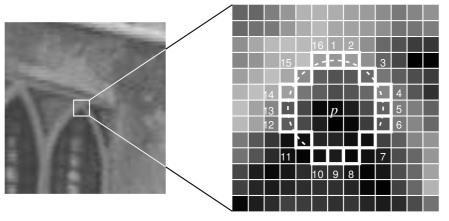
\includegraphics[scale=0.8]{images/fast01}
\caption{Detector FAST. Fonte \cite{FAST} }
\label{fig:fast01}
\end{figure}


Na imagem~\ref{fig:fast01} foi escolhido n=12 e seguido o seguinte algoritmo:
\begin{enumerate}
	\item Selecionar o ponto e testar primeiro as extremidades. No caso da imagem,
	escolhido o ponto p
	\item Comparar os pontos 1 e 9, e verificar se o ponto p tem intensidade
	com diferen�a de m�dulo t, ou seja os pontos 1 e 9 s�o mais claros ou mais escuros do que o ponto p pelo fator de t
	\item Avaliar se o ponto p continua sendo um candidato considerando os pontos 5
	e 13
	\item Analisar se p � uma aresta, sendo que para isso, pelo menos 3 desses
	pontos devem ser mais brilhantes ou mais escuros do que p, para que ent�o o
	teste pode ser feito nos demais pontos.
\end{enumerate}

